\documentclass{ximera}

%\usepackage{todonotes}

\newcommand{\todo}{}

\usepackage{esint} % for \oiint
\ifxake%%https://math.meta.stackexchange.com/questions/9973/how-do-you-render-a-closed-surface-double-integral
\renewcommand{\oiint}{{\large\bigcirc}\kern-1.56em\iint}
\fi


\graphicspath{
  {./}
  {ximeraTutorial/}
  {basicPhilosophy/}
  {functionsOfSeveralVariables/}
  {normalVectors/}
  {lagrangeMultipliers/}
  {vectorFields/}
  {greensTheorem/}
  {shapeOfThingsToCome/}
  {dotProducts/}
  {partialDerivativesAndTheGradientVector/}
  {../productAndQuotientRules/exercises/}
  {../normalVectors/exercisesParametricPlots/}
  {../continuityOfFunctionsOfSeveralVariables/exercises/}
  {../partialDerivativesAndTheGradientVector/exercises/}
  {../directionalDerivativeAndChainRule/exercises/}
  {../commonCoordinates/exercisesCylindricalCoordinates/}
  {../commonCoordinates/exercisesSphericalCoordinates/}
  {../greensTheorem/exercisesCurlAndLineIntegrals/}
  {../greensTheorem/exercisesDivergenceAndLineIntegrals/}
  {../shapeOfThingsToCome/exercisesDivergenceTheorem/}
  {../greensTheorem/}
  {../shapeOfThingsToCome/}
  {../separableDifferentialEquations/exercises/}
  {vectorFields/}
}

\newcommand{\mooculus}{\textsf{\textbf{MOOC}\textnormal{\textsf{ULUS}}}}

\usepackage{tkz-euclide}
\usepackage{tikz}
\usepackage{tikz-cd}
\usetikzlibrary{arrows}
\tikzset{>=stealth,commutative diagrams/.cd,
  arrow style=tikz,diagrams={>=stealth}} %% cool arrow head
\tikzset{shorten <>/.style={ shorten >=#1, shorten <=#1 } } %% allows shorter vectors

\usetikzlibrary{backgrounds} %% for boxes around graphs
\usetikzlibrary{shapes,positioning}  %% Clouds and stars
\usetikzlibrary{matrix} %% for matrix
\usepgfplotslibrary{polar} %% for polar plots
\usepgfplotslibrary{fillbetween} %% to shade area between curves in TikZ
%\usetkzobj{all}
\usepackage[makeroom]{cancel} %% for strike outs
%\usepackage{mathtools} %% for pretty underbrace % Breaks Ximera
%\usepackage{multicol}
\usepackage{pgffor} %% required for integral for loops



%% http://tex.stackexchange.com/questions/66490/drawing-a-tikz-arc-specifying-the-center
%% Draws beach ball
\tikzset{pics/carc/.style args={#1:#2:#3}{code={\draw[pic actions] (#1:#3) arc(#1:#2:#3);}}}



\usepackage{array}
\setlength{\extrarowheight}{+.1cm}
\newdimen\digitwidth
\settowidth\digitwidth{9}
\def\divrule#1#2{
\noalign{\moveright#1\digitwidth
\vbox{\hrule width#2\digitwidth}}}




% \newcommand{\RR}{\mathbb R}
% \newcommand{\R}{\mathbb R}
% \newcommand{\N}{\mathbb N}
% \newcommand{\Z}{\mathbb Z}

\newcommand{\sagemath}{\textsf{SageMath}}


%\renewcommand{\d}{\,d\!}
%\renewcommand{\d}{\mathop{}\!d}
%\newcommand{\dd}[2][]{\frac{\d #1}{\d #2}}
%\newcommand{\pp}[2][]{\frac{\partial #1}{\partial #2}}
% \renewcommand{\l}{\ell}
%\newcommand{\ddx}{\frac{d}{\d x}}

% \newcommand{\zeroOverZero}{\ensuremath{\boldsymbol{\tfrac{0}{0}}}}
%\newcommand{\inftyOverInfty}{\ensuremath{\boldsymbol{\tfrac{\infty}{\infty}}}}
%\newcommand{\zeroOverInfty}{\ensuremath{\boldsymbol{\tfrac{0}{\infty}}}}
%\newcommand{\zeroTimesInfty}{\ensuremath{\small\boldsymbol{0\cdot \infty}}}
%\newcommand{\inftyMinusInfty}{\ensuremath{\small\boldsymbol{\infty - \infty}}}
%\newcommand{\oneToInfty}{\ensuremath{\boldsymbol{1^\infty}}}
%\newcommand{\zeroToZero}{\ensuremath{\boldsymbol{0^0}}}
%\newcommand{\inftyToZero}{\ensuremath{\boldsymbol{\infty^0}}}



% \newcommand{\numOverZero}{\ensuremath{\boldsymbol{\tfrac{\#}{0}}}}
% \newcommand{\dfn}{\textbf}
% \newcommand{\unit}{\,\mathrm}
% \newcommand{\unit}{\mathop{}\!\mathrm}
% \newcommand{\eval}[1]{\bigg[ #1 \bigg]}
% \newcommand{\seq}[1]{\left( #1 \right)}
% \renewcommand{\epsilon}{\varepsilon}
% \renewcommand{\phi}{\varphi}


% \renewcommand{\iff}{\Leftrightarrow}

% \DeclareMathOperator{\arccot}{arccot}
% \DeclareMathOperator{\arcsec}{arcsec}
% \DeclareMathOperator{\arccsc}{arccsc}
% \DeclareMathOperator{\si}{Si}
% \DeclareMathOperator{\scal}{scal}
% \DeclareMathOperator{\sign}{sign}


%% \newcommand{\tightoverset}[2]{% for arrow vec
%%   \mathop{#2}\limits^{\vbox to -.5ex{\kern-0.75ex\hbox{$#1$}\vss}}}
% \newcommand{\arrowvec}[1]{{\overset{\rightharpoonup}{#1}}}
% \renewcommand{\vec}[1]{\arrowvec{\mathbf{#1}}}
% \renewcommand{\vec}[1]{{\overset{\boldsymbol{\rightharpoonup}}{\mathbf{#1}}}}

% \newcommand{\point}[1]{\left(#1\right)} %this allows \vector{ to be changed to \vector{ with a quick find and replace
% \newcommand{\pt}[1]{\mathbf{#1}} %this allows \vec{ to be changed to \vec{ with a quick find and replace
% \newcommand{\Lim}[2]{\lim_{\point{#1} \to \point{#2}}} %Bart, I changed this to point since I want to use it.  It runs through both of the exercise and exerciseE files in limits section, which is why it was in each document to start with.

% \DeclareMathOperator{\proj}{\mathbf{proj}}
% \newcommand{\veci}{{\boldsymbol{\hat{\imath}}}}
% \newcommand{\vecj}{{\boldsymbol{\hat{\jmath}}}}
% \newcommand{\veck}{{\boldsymbol{\hat{k}}}}
% \newcommand{\vecl}{\vec{\boldsymbol{\l}}}
% \newcommand{\uvec}[1]{\mathbf{\hat{#1}}}
% \newcommand{\utan}{\mathbf{\hat{t}}}
% \newcommand{\unormal}{\mathbf{\hat{n}}}
% \newcommand{\ubinormal}{\mathbf{\hat{b}}}

% \newcommand{\dotp}{\bullet}
% \newcommand{\cross}{\boldsymbol\times}
% \newcommand{\grad}{\boldsymbol\nabla}
% \newcommand{\divergence}{\grad\dotp}
% \newcommand{\curl}{\grad\cross}
%\DeclareMathOperator{\divergence}{divergence}
%\DeclareMathOperator{\curl}[1]{\grad\cross #1}
% \newcommand{\lto}{\mathop{\longrightarrow\,}\limits}

% \renewcommand{\bar}{\overline}

\colorlet{textColor}{black}
\colorlet{background}{white}
\colorlet{penColor}{blue!50!black} % Color of a curve in a plot
\colorlet{penColor2}{red!50!black}% Color of a curve in a plot
\colorlet{penColor3}{red!50!blue} % Color of a curve in a plot
\colorlet{penColor4}{green!50!black} % Color of a curve in a plot
\colorlet{penColor5}{orange!80!black} % Color of a curve in a plot
\colorlet{penColor6}{yellow!70!black} % Color of a curve in a plot
\colorlet{fill1}{penColor!20} % Color of fill in a plot
\colorlet{fill2}{penColor2!20} % Color of fill in a plot
\colorlet{fillp}{fill1} % Color of positive area
\colorlet{filln}{penColor2!20} % Color of negative area
\colorlet{fill3}{penColor3!20} % Fill
\colorlet{fill4}{penColor4!20} % Fill
\colorlet{fill5}{penColor5!20} % Fill
\colorlet{gridColor}{gray!50} % Color of grid in a plot

\newcommand{\surfaceColor}{violet}
\newcommand{\surfaceColorTwo}{redyellow}
\newcommand{\sliceColor}{greenyellow}




\pgfmathdeclarefunction{gauss}{2}{% gives gaussian
  \pgfmathparse{1/(#2*sqrt(2*pi))*exp(-((x-#1)^2)/(2*#2^2))}%
}


%%%%%%%%%%%%%
%% Vectors
%%%%%%%%%%%%%

%% Simple horiz vectors
\renewcommand{\vector}[1]{\left\langle #1\right\rangle}


%% %% Complex Horiz Vectors with angle brackets
%% \makeatletter
%% \renewcommand{\vector}[2][ , ]{\left\langle%
%%   \def\nextitem{\def\nextitem{#1}}%
%%   \@for \el:=#2\do{\nextitem\el}\right\rangle%
%% }
%% \makeatother

%% %% Vertical Vectors
%% \def\vector#1{\begin{bmatrix}\vecListA#1,,\end{bmatrix}}
%% \def\vecListA#1,{\if,#1,\else #1\cr \expandafter \vecListA \fi}

%%%%%%%%%%%%%
%% End of vectors
%%%%%%%%%%%%%

%\newcommand{\fullwidth}{}
%\newcommand{\normalwidth}{}



%% makes a snazzy t-chart for evaluating functions
%\newenvironment{tchart}{\rowcolors{2}{}{background!90!textColor}\array}{\endarray}

%%This is to help with formatting on future title pages.
\newenvironment{sectionOutcomes}{}{}



%% Flowchart stuff
%\tikzstyle{startstop} = [rectangle, rounded corners, minimum width=3cm, minimum height=1cm,text centered, draw=black]
%\tikzstyle{question} = [rectangle, minimum width=3cm, minimum height=1cm, text centered, draw=black]
%\tikzstyle{decision} = [trapezium, trapezium left angle=70, trapezium right angle=110, minimum width=3cm, minimum height=1cm, text centered, draw=black]
%\tikzstyle{question} = [rectangle, rounded corners, minimum width=3cm, minimum height=1cm,text centered, draw=black]
%\tikzstyle{process} = [rectangle, minimum width=3cm, minimum height=1cm, text centered, draw=black]
%\tikzstyle{decision} = [trapezium, trapezium left angle=70, trapezium right angle=110, minimum width=3cm, minimum height=1cm, text centered, draw=black]


\title{Law of Sines}

\begin{document}

\begin{abstract}
proportionalities
\end{abstract}
\maketitle











$\blacktriangleright$  \textbf{\textcolor{blue!55!black}{Acute Triangles}}  

An acute triangle is one where all three interior angles measure less than $90^{\circ}$. \\

In the diagram below, we drop an \textbf{altitude} from the top corner (angle $C$). This altitude (length $h$) is perpendicular to the opposite side, forming two right triangles inside the acute triangle.


\begin{image}[3in]
    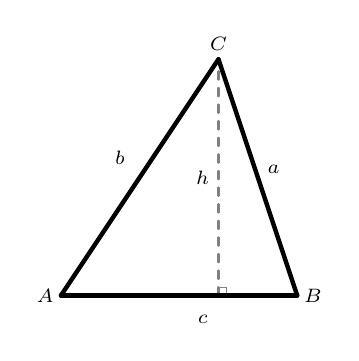
\begin{tikzpicture}[line cap=round]


    \draw [thick, dashed, gray] (2,0) -- (2,3);
    \draw [thin, gray] (2,0.1) -- (2.1,0.1);
    \draw [thin, gray] (2.1,0) -- (2.1,0.1);

	\draw [ultra thick] (0,0) -- (3,0);
	\draw [ultra thick] (3,0) -- (2,3);
	\draw [ultra thick] (0,0) -- (2,3);

 	


	\draw (2.7,1.6) node {\scriptsize{$a$}};
	\draw (0.75,1.75) node {\scriptsize{$b$}};
	\draw (1.8,-0.3) node {\scriptsize{$c$}};
	\draw (1.8,1.5) node {\scriptsize{$h$}};


	\draw (-0.2,0) node {\scriptsize{$A$}};
	\draw (3.2,0) node {\scriptsize{$B$}};
	\draw (2,3.2) node {\scriptsize{$C$}};


    \end{tikzpicture}
  \end{image}

From these two right triangles we can deduce the following. \\

\[    \frac{h}{b} = \sin(A)   \, \text{ and } \,    \frac{h}{a} = \sin(B)       \]



\[    h = b \sin(A)      \, \text{ and } \,    h = a \sin(B)    \]

\[     b \sin(A)  = a \sin(B)    \]


\[    \frac{\sin(A)}{a} = \frac{\sin(B)}{b}      \]




The same argument with an altitude from angle $B$ to side $b$ shows a similar relationship with angle $C$, giving us








\[    \frac{\sin(A)}{a} = \frac{\sin(B)}{b}  = \frac{\sin(C)}{c}    \]
















$\blacktriangleright$  \textbf{\textcolor{blue!55!black}{Obtuse Triangles}}   

An obtuse triangle is one with one angle greater than $90^{\circ}$. \\

We can establish the same relationship with an altitude on the outside.








\begin{image}[3in]
    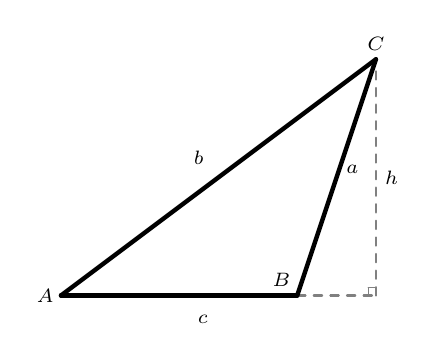
\begin{tikzpicture}[line cap=round]


    \draw [thick, dashed, gray] (4,0) -- (4,3);
    \draw [thick, dashed, gray] (3,0) -- (4,0);
    \draw [thin, gray] (4,0.1) -- (3.9,0.1);
    \draw [thin, gray] (3.9,0) -- (3.9,0.1);

	\draw [ultra thick] (0,0) -- (3,0);
	\draw [ultra thick] (3,0) -- (4,3);
	\draw [ultra thick] (0,0) -- (4,3);

 	


	\draw (3.7,1.6) node {\scriptsize{$a$}};
	\draw (1.75,1.75) node {\scriptsize{$b$}};
	\draw (1.8,-0.3) node {\scriptsize{$c$}};
	\draw (4.2,1.5) node {\scriptsize{$h$}};


	\draw (-0.2,0) node {\scriptsize{$A$}};
	\draw (2.8,0.2) node {\scriptsize{$B$}};
	\draw (4,3.2) node {\scriptsize{$C$}};


    \end{tikzpicture}
  \end{image}











\textbf{Note:}  Straight angles measure $180^{\circ}$.  $\angle B$ is part of a straight angle, which makes the measurement of the angle on the other side $180^{\circ} - B$. \\

\textbf{Additional Note:} The $y$-coordinates are the same as you move down the unit circle on either side from $90^{\circ}$.  Therefore, $\sin(180^{\circ} - B) = \sin(B)$ \\




\[    \frac{h}{b} = \sin(A)   \, \text{ and } \,    \frac{h}{a} = \sin(180^{\circ} - B)  = \sin(B)      \]



\[    h = b \sin(A)      \, \text{ and } \,    h = a \sin(B)    \]

\[     b \sin(A)  = a \sin(B)    \]


\[    \frac{\sin(A)}{a} = \frac{\sin(B)}{b}      \]




The same argument could be made with angle $C$, giving us








\[    \frac{\sin(A)}{a} = \frac{\sin(B)}{b}  = \frac{\sin(C)}{c}    \]






\begin{theorem}  \textbf{\textcolor{green!50!black}{Law of Sines}} 



For any triangle with angles $A$, $B$, and $C$, and opposite sides $a$, $b$, and $c$, respectively, 


\[    \frac{\sin(A)}{a} = \frac{\sin(B)}{b}  = \frac{\sin(C)}{c}    \]


\end{theorem}





\begin{example}  General Triangles \\

Suppose we have a triangle with $A=46^{\circ}$, $B=65^{\circ}$, and $a=14$.

Figure out the other three measurements. (3 decimals)


\begin{explanation}

$A + B + C = 46^{\circ} + 65^{\circ} + C = \answer{180}^{\circ}$ \\

$C = \answer{69}^{\circ}$


$\frac{\sin(46^{\circ})}{14} = \frac{\sin(65^{\circ})}{b}$

$b = \frac{14 \sin(65^{\circ})}{\sin(46^{\circ})} \approx \answer[tolerance=0.001]{17.63882523}$

$\frac{\sin(46^{\circ})}{14} = \frac{\sin(69^{\circ})}{c}$

$c = \frac{14 \sin(69^{\circ})}{\sin(46^{\circ})} \approx \answer[tolerance=0.001]{18.16961325}$

\end{explanation}


\end{example}












\begin{example}  No Triangle \\

Suppose we have a triangle with $C=55^{\circ}$, $a=4$, and $c=2$.

Figure out the other three measurements.


\begin{explanation}


$\frac{\sin(55^{\circ})}{2} = \frac{\sin(A)}{4}$

$\sin(A) = \frac{4 \sin(55^{\circ})}{2} \approx 1.638304086$

This is greater than $1$. $\sin(A)$ cannot be greater than $1$.

Therefore, there is no triangle with $C=55^{\circ}$, $a=4$, and $c=2$. 

\end{explanation}


\end{example}












\begin{example}  Two Triangles \\

Suppose we have a triangle with $A=37^{\circ}$, $a=12$, and $b=16$.

Figure out the other three measurements.


\begin{explanation}


$\frac{\sin(37^{\circ})}{12} = \frac{\sin(B)}{16}$

$\sin(B) = \frac{16 \sin(37^{\circ}}{12}) \approx \answer[tolerance=0.001]{0.8024200309}$

There are two angles whose sine is $0.8024200309$. One in the first quadrant and one in the second quadrant. \\

Therefore, there are two triangles with $A=37^{\circ}$, $a=12$, and $b=16$. 

Using the calculator, the two angles are

\begin{itemize}
\item $B \approx SIN^{-1}(0.8024200309) \approx \answer[tolerance=0.01]{53.36}^{\circ}$
\item $B \approx 180^{\circ} - 53.36^{\circ} = 126.64^{\circ}$
\end{itemize}

\end{explanation}


\end{example}














\begin{center}
\textbf{\textcolor{green!50!black}{ooooo-=-=-=-ooOoo-=-=-=-ooooo}} \\

more examples can be found by following this link\\ \link[More Examples of Triangles]{https://ximera.osu.edu/csccmathematics/precalculus2/precalculus2/generalTriangles/examples/exampleList}

\end{center}





\end{document}
